\subsection{H1-hESC cell line} \label{meth-encode-h1-subsect}
The same experiment was conducted for clustering DNA methylation profiles for the H1-hESC cell line. As promoter regions were considered 1000bp upstream and 1000bp downstream of the TSS, resulting in 2000bp in total. This resulted in 5,520 promoter regions for testing. The total number of clusters K was set to 5, and the methylation profiles were modelled using $5^{th}$ degree polynomials. 

Similarly to \emph{Fig. \ref{meth-k562-pic}} above, figures \emph{\ref{methH1:first}} and \emph{\ref{methH1:second}} depict the five methylation profiles that are fitted to the promoter regions of the H1-hESC data, and the corresponding expression levels of the protein coding genes assigned to each cluster K, respectively. About 70\% of the promoter regions were assigned to cluster K=4 (\emph{red curve}), 13\% to cluster K=5 (\emph{green curve}), and the remaining clusters had around the same percentage of assignments. 

Comparing to the K562 cell line, we observe similar functional role of the methylation profiles for the H1-hESC cell line. That is, unmethylated (\emph{red curve}) and U-shape (\emph{green curve}) promoter regions tend to have higher transcription activity, while hyper-methylated promoter regions (\emph{blue curve}) tend to have low expression levels. Finally, for both K562 and H1-hESC cells, promoter profiles that become methylated right after the TSS (\emph{black curve}) tend to silence gene expression. 

In general, we see that gene expression levels for the H1-hESC cells are higher than the K562 cells. This could be due to different biological conditions. For example, the K562 cells are \emph{cancer} cells, thus epigenetic modifications, such as alterations in CpG methylation patterns and histone modifications, would result in silencing certain genes and activating oncogenes. The current project is not concerned in analysing and comparing different cell lines, but is mainly concentrated in finding methylation patterns that regulate gene expression, such as activating or inhibiting transcription. 

\begin{figure}[ht!]
     \begin{center}
        \subfigure[]{
            \label{methH1:first}
            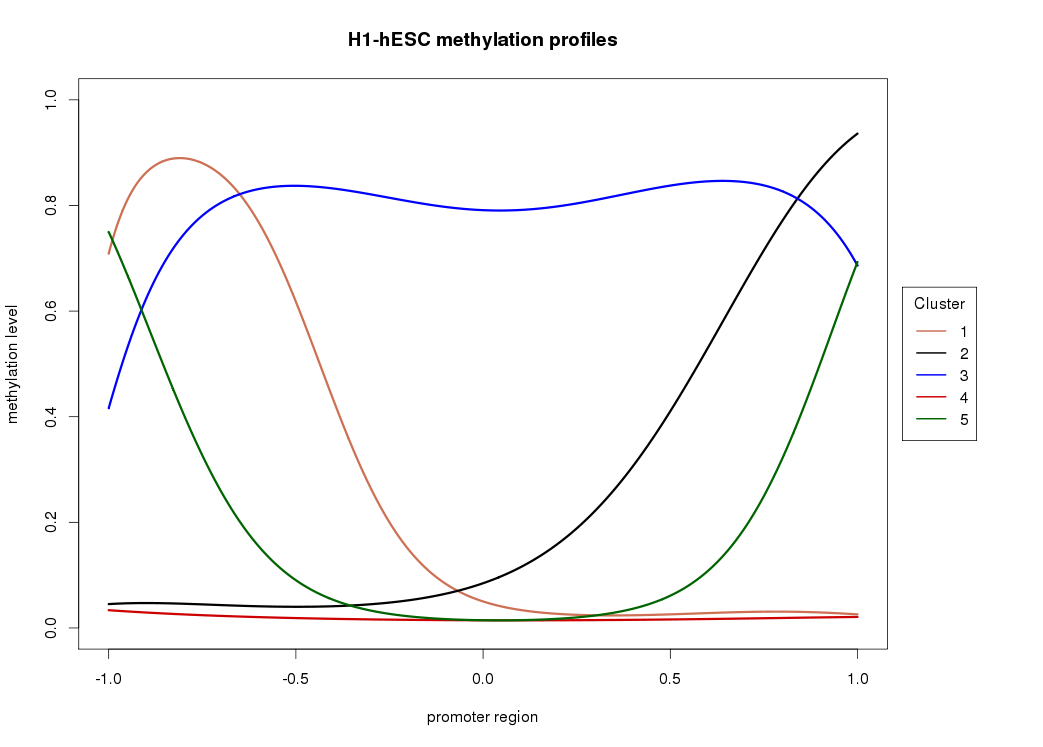
\includegraphics[width=0.45\textwidth]{images/h1MethProfClusters}
        }
        \subfigure[]{
           \label{methH1:second}
           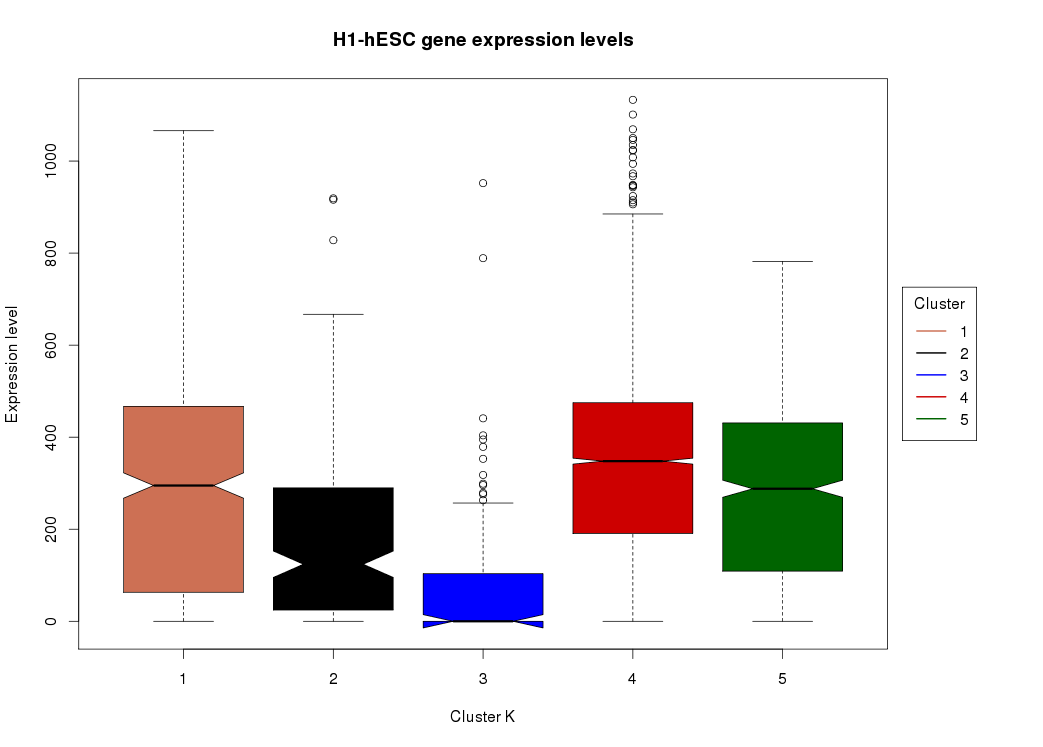
\includegraphics[width=0.495\textwidth]{images/h1MethProfBoxPlot}
        }
    \end{center}
    \caption{\emph{(a) Clustering DNA methylation profiles for the H1-hESC cell line with $5^{th}$ degree polynomial, each colour represents a different cluster. (b) Boxplot with the corresponding gene expression levels of the protein-coding genes assigned to each cluster K for the H1-hESC cell line. See the text for details.}}
   \label{meth-H1-pic}
\end{figure}